\begin{infocard}{Áreas de polígonos regulares}
    \begin{minipage}{.6\textwidth}
        Considere un polígono regular $ABCDEF$ inscrito en un círculo O, $\overline{OA}$ y $\overline{OB}$  son los radios del centro del círculo O hacia los dos vértices del hexágono. $\overline{OG}$ esta dibujado del centro del polígono regular perpendicular al lado del polígono. Así, $\overline{OG}$ es un apotema.

        Si un polígono regular de $n$ lados, de longitud L, tiene un área $A$ de unidades cuadradas, un perímetro de $P$ unidades, un apotema de $a$ unidades, entonces el área es un medio del producto del perímetro y el apotema:

        \[A=\dfrac{nLa}{2}\]

        donde el perímetro es \[P=nL\]
    \end{minipage}\hfill
    \begin{minipage}{.3\textwidth}
        \begin{figure}[H]
            \centering
            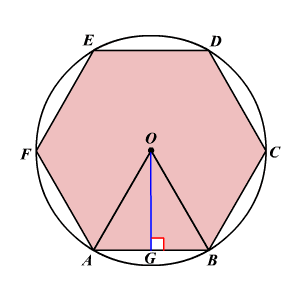
\includegraphics[width=0.9\linewidth]{../images/apothem}
            \caption{Hexágono regular para demostración.}
            \label{fig:}
        \end{figure}
    \end{minipage}

\end{infocard}
